\documentclass[10pt]{article}
\usepackage{pdfpages}
\usepackage[utf8]{inputenc}
\usepackage{graphicx}
\usepackage{hyperref}
\usepackage{fontenc}
\usepackage{mathptmx}
\usepackage{geometry}
\usepackage{titling}
\setlength{\topskip}{0mm}
\setlength{\droptitle}{-8em} 

\title{{\large \textbf{CONCORDIA UNIVERSITY \\ DEPARTMENT OF COMPUTER SCIENCE AND SOFTWARE ENGINEERING \\ SOEN 6481: SOFTWARE SYSTEM REQUIREMENTS SPECIFICATION \\ SECTION WW WINTER 2019 \\ Irrational number: Champernowne Constant ($C_{10}$)}  \\ }}
\author{\normalsize \textbf {STUDENT NAME: YONGCONG LEI} \\ \normalsize \textbf{STUDENT IDENTIFICATION NUMBER: 40045701 }}
\date{}
\begin{document}
\maketitle

\section{Characteristics}
\paragraph{}
Champernowne Constant $C_{10}$ is a transcendental real constant whose decimal expansion has import properties. The constant is named because economist and mathematician D. G. Champernowne published it in 1933.

\paragraph{}
The first interesting property of Champernowne Constant is that the number is defined by combination of successive base-10 integers, which means $C_{10} = 0.12345678910111213141516…$.

\paragraph{}
Besides, it's also a transcendental numbers. All real transcendental numbers are irrational numbers, but not all irrational numbers are transcendental. The property of transcendental also makes Champernowne Constant uncountable infinite. However, $C_{10}$ is computable  although it is a transcendental number, which means that we can write a program to compute it with any desired precision.

\paragraph{}
What's more, Champernowne number was proved normal in base 10. The fact shows all of its digits being equally likely, All pairs of digits being equally likely, All triplets of digits being equally likely, etc. For example, we can find that string $[0], [1], ..., [9]$ are equally distributed in the constant at rate of 1/10, and $ [0,0],[0,1],...,[9,8],[9,9]$ are equally distributed at rate of 1/100.

\pagebreak
\section{Interview}
My interviewee is my roommate. He has a background of mathematics, which might be useful for understanding the constant and coming up an idea of what the constant is about, why we need this constant and what kind of scenario in which the constant might be helpful.
\subsection{Questions}
\begin{enumerate}
    \item Are there any other Champernowne Constant with different bases?
    \item Do you think Champernowne Constant in useful in our programming?
    \item How can we get a transcendental numbers based on the Champernowne Constant?
    \item What's the property of Champernowne that might be useful in problem? 
    \item Please give an example of application that might use the Champernowne Constant.
\end{enumerate}
\subsection{Response}
\begin{enumerate}
    \item Yes. $C_{10}$ is only one of the Champernowne Constant in its family. As the equation shows, the constant is based on 10. There are other Champernowne Constant with other bases. For example, $C_{2}$ is a constant with binary sequence, while $C_16$ is a hexadecimal Champernowne constant.
    \item Not exactly. There is a pattern in Champernowne Constant, which makes it easy to get the constant in arbitrary length. In other words, it's easy to write a program to generate a Champernowne Constant of length L with base N. L is a number that is greater than or equal with 1 and N is number that is greater than or equal with 2.
    \item Actually, Any non-constant algebraic function of a single variable yields a transcendental value when applied to a transcendental argument. For example, we can get a new transcendental number by multiplying a constant value to $C_{10}$, which is $$\texttt{new transcendental number} = C_{10} * N \texttt { (N is a constant)}$$.
    \item The normality of Champernowne Constant might be useful in some practical problems. The property is interesting. It means if we number pick a digit in $C_{10}$, the possibility of picking a number from 0 to 10 is equal. If we pick two digits in $C_{10}$, the possibility of picking a number from 0 to 99 is equal. If we pick three digits in $C_{10}$, the possibility of picking a number from 0 to 999 is equal, etc.
    \item The interviewee didn't give an specific example for this question. He thinks although there are some interesting properties about Champernowne Constant, it's not really helpful in practice. Maybe we can make use of its normality on some algorithms which is used for random number generation. However, he was not clear about it.
\end{enumerate}
\subsection{Analysis}
By having the interview with my roommate, I have a better understanding of Champernowne Constant. As he said, although there are some interesting properties about Champernowne Constant, it's not really helpful in practice. It's just one of the pretty number that people (especially in mathematics field) thought would be good to experiment with. The pattern of the constant is clear since it is constructed in such a way that its (decimal) digits are easy to investigate.

\section{Persona}
\includepdf[]{image/persona.pdf}

\section{Problem Domain Model}
\subsection{Relevant concept}
    
\begin{enumerate}
    \item There would be at most one user of calculator at certain time. There should not be two users using the calculator at the same time. 
    \item Each calculator should provide the functionality for user to input data. The functionality is provided with keyboard in our case.
    \item There are different kinds of input unit for a calculator, such as digits, sign (negative/positive), constant etc.
    \item Each calculator should provide the functionality to output the result of calculation. Specifically, it should be output to console in our case.
    \item Each calculator can support multiple operators, including binary operators and unary operators.
\end{enumerate}

\begin{center}
  \begin{figure}[h!]
      \centering
      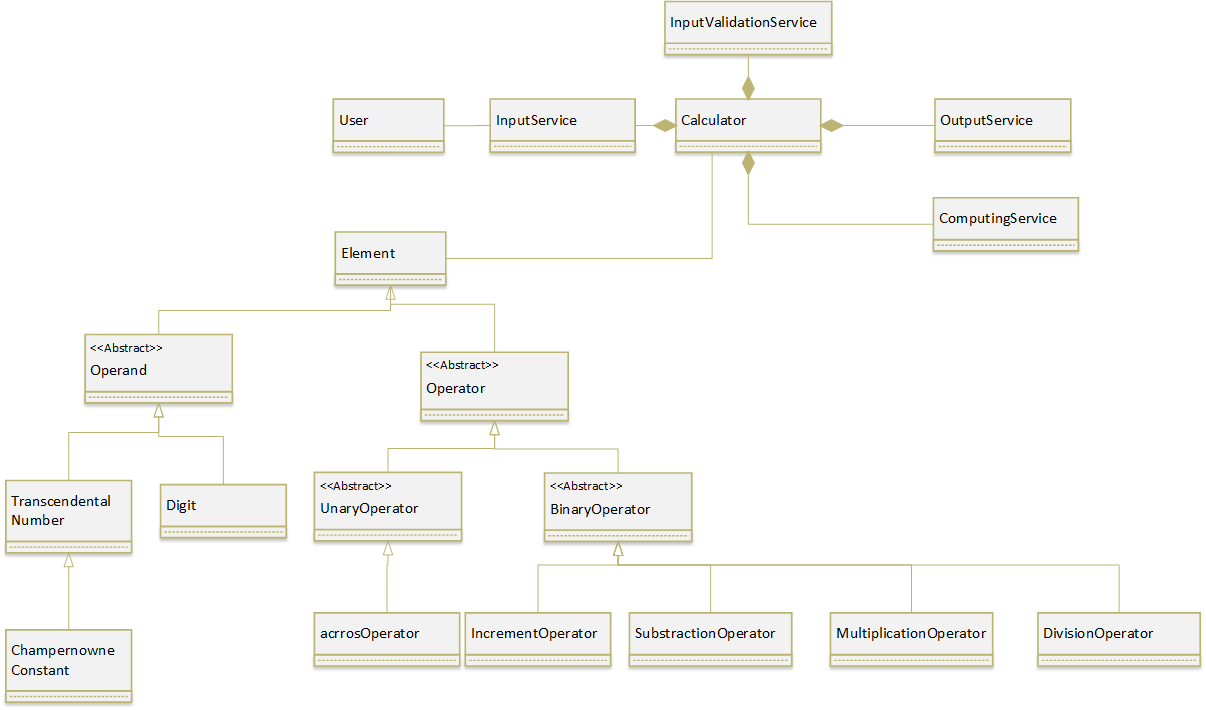
\includegraphics[width=0.9\linewidth]{image/domain model.png}
      \caption{Domain model diagram}
      \label{fig:my_label}
  \end{figure}
\end{center}


\pagebreak
\section{Use Case Model}
\begin{enumerate}
    \item A user need to turn on the calculator at first.
    \item A user can turn off the calculator after using it.
    \item A user can input a sequence of operands and operators and he should be able to see what he input.
    \item A user can delete an operand or operator which he input and he should be able to see the change.
    \item A user can submit the sequence and get the result if the sequence is valid
    \item A user can reset the calculator to start another operation.
    \item A user can show the sequence and result of last calculation.
    \item A user can get a second transcendental number based on Champernowne Constant
\end{enumerate}

Figure 2 is the use case diagram of the calculator. A use case stands head and it indicates one of the possible use of Champernowne Constant. 

Figure 3 is the sequence diagram of the calculator. It shows the sequence from use input to calculator output.

\begin{center}
  \begin{figure}[h!]
      \centering
      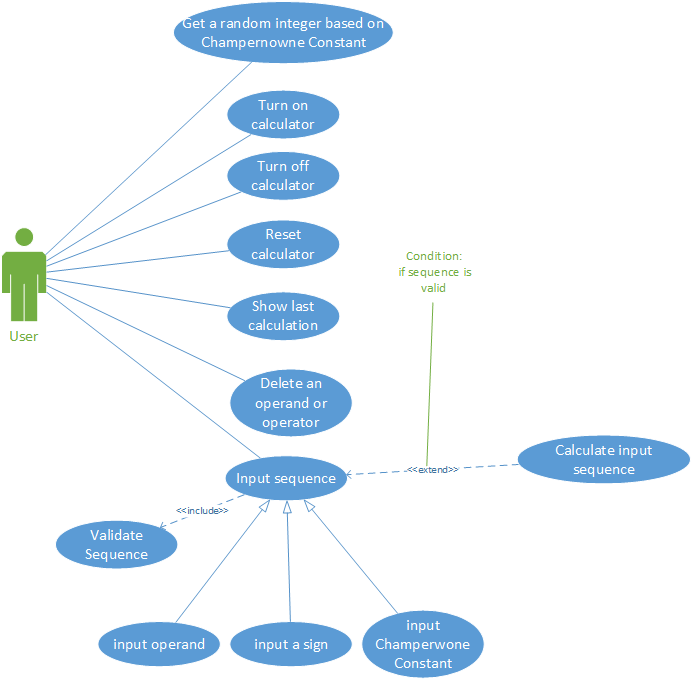
\includegraphics[width=0.9\linewidth]{image/useCaseDiagram.png}
      \caption{Use case diagram}
      \label{fig:my_label}
  \end{figure}
\end{center}

\begin{center}
  \begin{figure}[h!]
      \centering
      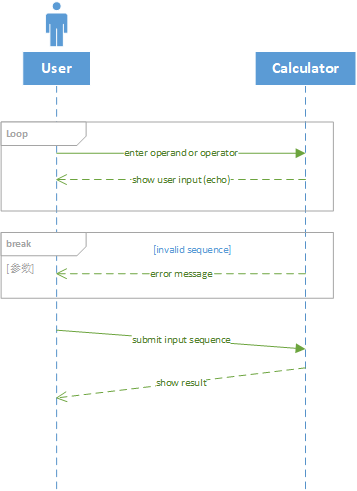
\includegraphics[width=0.7\linewidth]{image/sequenceDiagram.png}
      \caption{sequence diagram}
      \label{fig:my_label}
  \end{figure}
\end{center}

\end{document}
